\section{Results and Discussion}
\subsection{RQ1: Checkpoint Selection and Training Changes}
\begin{table}[t]
\caption{Historical clean mAP (\%). Best means minimum validation loss. R1/R2 best use archived BF16-backbone evaluations; final rows are the new FP32 cosine baselines.}
\label{tab:checkpoints}
\centering\footnotesize
\begin{tabular}{lrrr}
\toprule
Checkpoint & Epoch & Oxford & Paris \\
\midrule
\checkpointrows
\bottomrule
\end{tabular}
\end{table}

B0 best remains strongest on both clean benchmarks (Table~\ref{tab:checkpoints}), reaching 81.06\% on Oxford and 77.12\% on Paris. The best available historical evaluations for \Rone{} reach 79.53\% and 71.93\%; \Rtwo{} reaches 80.49\% and 72.76\%. The gate run is higher at these selected checkpoints, but this ordering reverses at epoch 100. Thus, the saved evidence does not support an unconditional benefit from the gate or superiority of either new run over B0.

\begin{figure*}[t]
\centering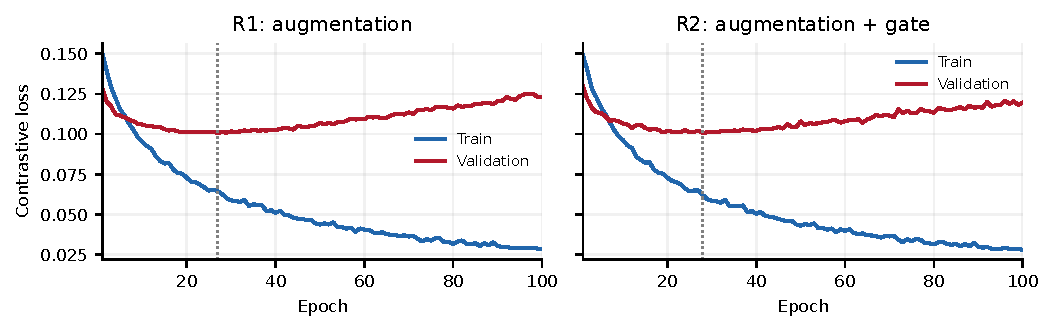
\includegraphics[width=0.92\textwidth]{training.pdf}
\caption{Training and validation contrastive loss for the two new runs. Dotted lines mark validation-selected epochs 27 and 28. Validation negatives depend on the current encoder; curves show the implemented monitoring objective.}
\label{fig:training}
\end{figure*}

The histories show late-training deterioration (Fig.~\ref{fig:training}). \Rone{} has minimum validation loss 0.100764 at epoch 27, rising to 0.123108 at epoch 100; \Rtwo{} rises from 0.100519 at epoch 28 to 0.119673. Meanwhile, training loss falls to approximately 0.0288 and 0.0280. Combined with lower final retrieval scores, this is consistent with overfitting. It does not isolate a single cause: optimization trajectory, augmentation, and changed precision/runtime are not independently controlled.

The archived B0 best epoch is 12, selected by validation, not by taking the best score separately on each benchmark. For example, B0's Paris score at epoch 8 is higher than at epoch 12, but substituting it would mix selection criteria. We preserve the declared checkpoint rule. Similarly, a lower validation loss across two runs is not automatically a calibrated estimate of better retrieval, particularly with changing mined negatives.

\subsection{RQ2: Search Improvements for Fixed Encoders}
\begin{table*}[t]
\caption{Main post-training results, mAP (\%). C denotes clean and R the mean over 18 corrupted-query conditions. Both encoders are fixed at epoch 100 and use FP32 extraction. These are exploratory comparisons against each encoder's own cosine baseline.}
\label{tab:post}
\centering\small
\begin{tabular}{lrrrrrrrr}
\toprule
& \multicolumn{4}{c}{\Rone{}: augmentation} & \multicolumn{4}{c}{\Rtwo{}: augmentation + gate} \\
\cmidrule(lr){2-5}\cmidrule(lr){6-9}
& \multicolumn{2}{c}{Oxford5k} & \multicolumn{2}{c}{Paris6k} & \multicolumn{2}{c}{Oxford5k} & \multicolumn{2}{c}{Paris6k} \\
Method & C & R & C & R & C & R & C & R \\
\midrule
\posttrainingrows
\bottomrule
\end{tabular}
\end{table*}

\paragraph{Expansion provides low-cost gains}
AQE and weighted QE improve both clean and corrupted mAP for both final encoders (Table~\ref{tab:post}). For \Rone, weighted QE increases Oxford clean from 74.00\% to 76.45\% and Paris clean from 64.29\% to 65.89\%. Equal-dataset corrupted mAP rises from 66.82\% to 69.34\%, a 2.52-percentage-point gain. AQE and weighted QE differ little, so these observations do not establish the necessity of similarity weighting.

The cosine gate opens for every measured query view and accepts ten feedback images, causing gated QE to equal weighted QE. This diagnostic is important: identical scores here indicate an inactive selection constraint, rather than evidence that the gate improves feedback reliability.

\paragraph{Geometry is most useful as a feedback filter}
For \Rone, local-match re-ranking reaches 78.53\% Oxford clean, exceeding the geometric-score re-ranker at 76.68\%. Geometric verification is therefore not uniformly stronger when used only to reorder a short prefix. In contrast, verified QE reaches 78.94\% and 66.97\% clean on Oxford and Paris, and 76.28\% and 65.82\% under corruption. Its corrupted dataset-macro mAP is 71.05\%, or 4.23 points above cosine. For \Rtwo, verified QE also gives the highest main-method mAP in all four columns: 76.85\%, 74.25\%, 65.10\%, and 64.31\%.

Verified feedback is not always available. Across clean and corrupted views, its gate opens for 88.39\% of \Rone{} Oxford cases and 92.96\% of Paris cases. The mean feedback counts, including closed gates, are 6.87 and 8.56. Fallbacks are retained rather than removing difficult queries from evaluation. These observations support examining feedback quality, but do not prove that the chosen homography criterion is optimal.

\begin{table}[t]
\caption{Two-encoder fusion, mAP (\%). Both use R1+R2 epoch 100; column order matches Table~\ref{tab:post}.}
\label{tab:fusion}
\centering\footnotesize
\begin{tabular}{lrrrr}
\toprule
& \multicolumn{2}{c}{Oxford} & \multicolumn{2}{c}{Paris} \\
Method & C & R & C & R \\
\midrule
\fusionrows
\bottomrule
\end{tabular}
\end{table}

\paragraph{Fusion does not beat the stronger encoder}
Neither score fusion nor RRF exceeds \Rone{} cosine on either clean dataset or their corrupted means (Table~\ref{tab:fusion}). Score fusion obtains 73.55\% Oxford clean and 64.04\% Paris clean, compared with 74.00\% and 64.29\% for \Rone. Complementary errors are a possible requirement for useful fusion, but we have not isolated error dependence as the cause. The experiment only establishes that these two encoders and combination rules do not improve the stronger single ranking.

\paragraph{Global graph diffusion degrades ranking}
Mutual diffusion reduces \Rone{} Oxford clean from 74.00\% to 48.95\%, and union diffusion to 23.67\%. Paris also deteriorates. This is not primarily explained by numerical failure: aggregate diagnostics report full convergence for both \Rone{} graphs, zero fallback, and mean iteration counts approximately 63--93. \Rtwo{} Oxford mutual diffusion reaches convergence in 99.77\% of views, with the remaining views retained at the iteration cap.

Propagation can reinforce misleading neighborhoods, but identifying the dominant mechanism would require additional analysis. A stable iterative result can still be a poor ranking. Our global graph, seeding, and fixed propagation parameters also differ from regional diffusion systems~\cite{diffusion}; no general rejection of diffusion follows.

\subsection{Corruption Severity and Exploratory Sensitivity}
\begin{figure*}[t]
\centering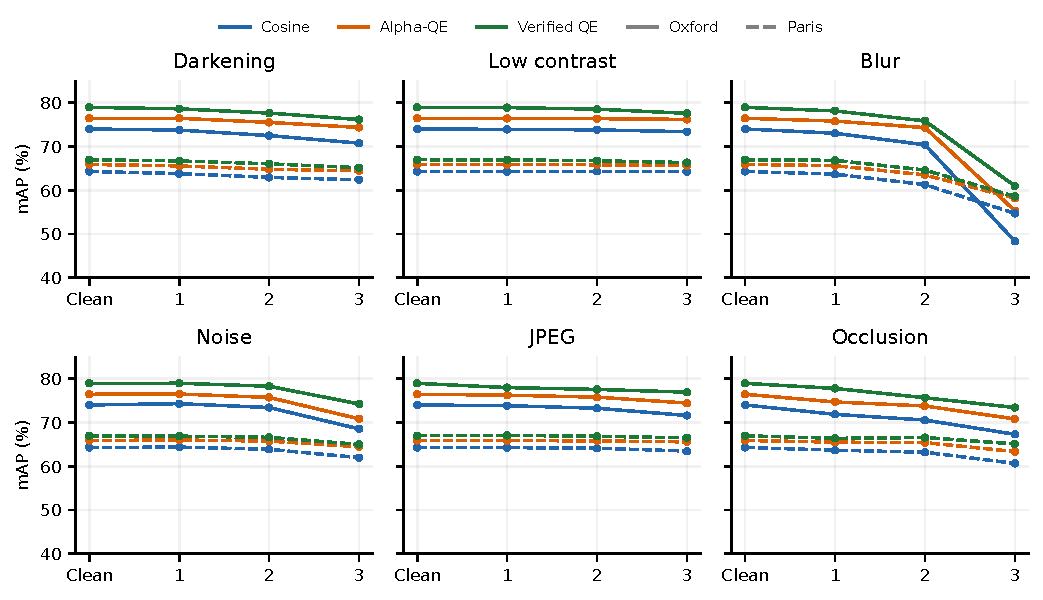
\includegraphics[width=0.96\textwidth]{robustness.pdf}
\caption{R1 retrieval under increasing query corruption. Solid curves: Oxford; dashed: Paris. Blue: cosine; orange: weighted QE; green: verified QE. Each non-clean point averages the prescribed realizations. The gallery is always clean.}
\label{fig:robustness}
\end{figure*}

Figure~\ref{fig:robustness} shows that severe blur is particularly damaging to \Rone. Its worst condition is blur severity three on both datasets: cosine mAP is 48.33\% Oxford and 54.71\% Paris. Verified QE raises those same condition scores to 60.97\% and 58.60\%, respectively. Improvements remain conditional on the starting encoder and the particular query transformations. A smaller clean-to-corrupted drop alone would not demonstrate a better system if absolute mAP were lower.

The suite partially overlaps training augmentation but is not identical. In particular, Gaussian noise is not included in the saved augmentation policy. Severe occlusion may remove identifying object content, and we do not claim that every generated query preserves perfect semantic observability. Results measure this defined stress test, not all natural distribution shifts.

Clean sensitivity contains 100 additional grouped evaluations, representing 5,500 per-query AP values. For instance, \Rone{} weighted QE with $\lambda=1$ reaches 77.30\% Oxford and 66.56\% Paris clean, above the frozen $\lambda=0.5$ setting. Local re-ranking with $K=100$ and $\eta=0.5$ reaches 78.85\% and 66.94\%. These are test-set observations, not independently validated parameter selections. They do not replace the main setting for corruption results. The complete configurations, including weaker variants, accompany the paper.

\subsection{RQ3: Quality--Latency Trade-offs}
\begin{figure*}[t]
\centering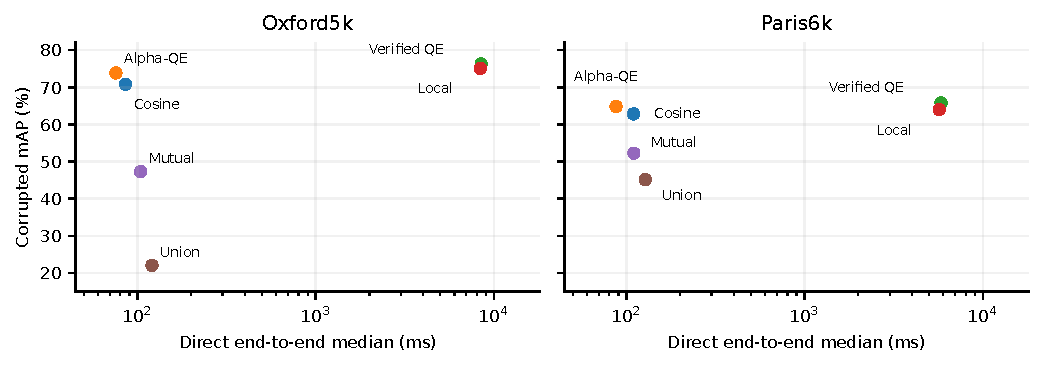
\includegraphics[width=0.96\textwidth]{quality_latency.pdf}
\caption{R1 corrupted mAP versus measured direct end-to-end median query latency (logarithmic horizontal axis). Quality uses the complete corruption suite; latency uses the predefined 28-sample subset. Offline gallery preparation is excluded.}
\label{fig:latency}
\end{figure*}

QE adds approximately 3--5 ms to retrieval-only processing for \Rone. Direct weighted-QE medians are 75.55 ms on Oxford and 87.34 ms on Paris. Verified QE has medians 8.48 s and 5.82 s; local matching and geometric processing dominate this scale of cost. These methods occupy substantially different deployment regimes (Fig.~\ref{fig:latency}).

The direct cosine medians for \Rone{} are 85.52 and 109.53 ms, larger than the corresponding weighted-QE medians despite QE's additional operation. The small, independently timed sample and execution variability prevent interpreting this ordering as a causal speed-up. Retrieval-only timings more directly expose the expansion overhead. We do not infer a speed improvement from the direct-median inversion.

Offline computation also matters. The shared local-feature cache reports approximately 2.56 GB of stored data. Its recorded builds take 2,464 s for Oxford and 3,049 s for Paris, covering gallery and query-view features. Query local features are nevertheless recomputed in the direct timer so cached queries do not hide online costs. Both fusion encoders must also be executed: direct score-fusion medians are 147.17 ms Oxford and 160.30 ms Paris. Its extra encoding cost does not yield an accuracy improvement here.

\subsection{Reproducibility and Limits of Inference}
The main grid has 20 ranking configurations per dataset: nine per encoder and two fusion rules. Across 110 queries and 31 views this yields 68,200 main AP records, with no missing cells in the saved coverage audit. Together with sensitivity, the saved per-query records total 73,700. Descriptors, rankings, image IDs, pixel checksums, checkpoint hashes, graph diagnostics, and job completion states identify the evaluated artifacts. Smoke checks cover export/reload consistency, finite descriptors, perfect/junk evaluator cases, QE identity and closed-gate behavior, single-ranker fusion, prefix-preserving re-ranking, and graph numerical behavior.

Only one training seed is available. The many corrupted views do not estimate variability across independent training runs, and we make no statistical-significance claim. Closely related landmark queries further limit interpretations based on treating all query views as independent observations. B0 lacks a matching corruption/post-training experiment, and the training histories differ in budget, precision, and runtime. Thus, the evidence supports fixed-encoder search gains and descriptive training observations, not a controlled attribution of gains or losses to augmentation or attention.
